
\documentclass{IOS-Book-Article}

\usepackage{mathptmx}
\usepackage{graphicx}
\usepackage{subfigure}

%\usepackage{times}
%\normalfont
%\usepackage[T1]{fontenc}
%\usepackage[mtplusscr,mtbold]{mathtime}
%
\begin{document}
\begin{frontmatter}              % The preamble begins here.

%\pretitle{Pretitle}
\title{D\&C Matrix Assembly Parallelisation for Unstructured Meshes}
\runningtitle{D\&C Assembly}
%\subtitle{Subtitle}

\author[A]{\fnms{Lo\"ic} \snm{Th\'ebault}%
\thanks{Corresponding Author E-mail: }},
\author[A]{\fnms{Eric} \snm{Petit}},
\author[B]{\fnms{Marc} \snm{Tchiboukdjian}},
and
\author[C]{\fnms{Quang} \snm{Dinh}}

\runningauthor{L. Th\'ebault et al.}
\address[A]{PRISM - University of Versailles, France}
\address[B]{Somwhere}
\address[C]{Dassault Aviation, Saint-Cloud, France}

\begin{abstract}
Current algorithms and runtimes struggle to scale to a large number of cores and show a poor parallel efficiency on current HPC machine.
The pure MPI codes are wasting IO, memory and communication. HPC users have to explore new paradigm to make an efficient usage of the new resources at their disposal.
Hybrid MPI+threads is one of them. In this paper we propose and evaluate a Divide \& Conquer, D\&C, approach for the parallelisation on shared memory of an unstructured mesh assembly to sparse matrix.
Our target application is an industrial CFD application from Dassault Aviation computing mesh deformation for structure optimization.
The implementation is based on the versatile cilk runtime and standard MPI. The original fortran code has been modified so that the elision of our modification is equivalent to the original, pure MPI, application.
Preliminary results on the first step of the application, the matrix assembly from mesh to CSR matrix storage format, are encouraging and show good locality and scalability characteristics.
\end{abstract}

\begin{keyword}
Divide and Conquer, Task, Cilk, Mesh Partitioning, CFD, Matrix Assembly 
\end{keyword}
\end{frontmatter}

\thispagestyle{empty}
\pagestyle{empty}

\section*{Introduction}

Positionment : code MPI compare to hybrid.\\
Problem on FEM : assembling, parallelization with shared memory non trivial.\\
Assembling on multicore, not on GPU (most of papers are for GPUs)\\\\

Current algorithms and runtimes struggle to scale on a large number of cores and show a poor parallel efficiency on current HPC machine. The main reason is that the runtimes
and algorithms are using large amount of global communication and synchronization. It causes a severe problem on an increasing number of nodes and core per nodes.
HPC users have to explore new paradigm to make an efficient usage of the new resources at their disposal. 
The major effects of the core count increase per node are a lower memory per core, higher requirement for concurrency (TLP, ILP, vector), higher coherency traffic and higher
cost for coherency protocol. The result is severe challenge for performance scalability. The many-core accelerators such has the Xeon Phi exacerbate even more these issues. 
In order to help the developer to make a better usage of the shared resources and mitigate the node scalability issue, we propose and evaluate a new parallelisation strategy 
 to exploit more efficiently the shared memory level for iterative method using unstructured meshes. The objective is to take advantage of the full topology of the machine and
 enhance the data and synchronization locality to release pressure on the distributed structure such as memory, network and global I/O. 

In this paper we evaluate the Divide and Conquer, D\&C, approach on  unstructured meshes. Our implementation is based on a task-based runtime, Cilk~\cite{cilk5}.
The rational is to divide recursively the work in two or more independent tasks, synchronize locally these tasks before returning. This recursive approach has many advantages.
First the recursive sharing naturally exposes high concurrency. As long as the application is large enough, it is possible to produce a deeper tree to get more concurrency
and therefore match the higher requirement of many-core system. Another advantages is the locality of synchronization, only nodes of a same parent node in the recursive
tree needs to be synchronized. And finally, it greatly improved the data locality by reordering the data in smaller independent sets. The D\&C approach is particularly
interesting for its ability to scale naturally to an increasing number of node thanks to its architecture oblivious concept.
Each leaves is responsible of its own data and there is a very minimal amount of sharing, avoiding costly locks and coherency protocols. 

We apply the d\&C strategy for the parallelisation of an industrial CFD code from Dassault Aviation computing the effect of mesh deformation to optimize the plane structure.
The process alterate the mesh geometry and be conservative of the mesh topology.  We have to work on a very unstructured mesh. Therefore, load balancing and interface
computation prevent us to use geometrical domain decomposition.
We use Metis~\cite{Metis} to do a topological domain decomposition that will not vary with the mesh deformation.
The application iterates over three basic steps:
\begin{itemize}
\item Edge matrix assembly to CSR storage from the mesh coordinate array. This step potentially needs MPI communication in the case of using the elastic version.
Explain in section ...
\item Solve ... ??? what?
\item Update the mesh coordinate and value, exchange the halo with other MPI rank.
\end{itemize}
Say somewhere that one of the major difficulty when parallelizing this numerical code is to be very conservative on the numerical result. explain shortly why and how we deal
with that.


Even if the final goal is to parallelize the full application, we focus first on the assembly part. Indeed, despite a limited time coverage, renumbering, reordering,
task tree structure because...Explain what is assembling and why this is difficult to parallelize



Paper outline
Section 1 presents rge application, its main characteristics and the test cases.
The second section present the divide and conquer approach to parallelization. 
Section 3 presents the implemention based on metis, silk and MPI.
Section 4 presents the result of performance and scalability. 
In section 4 we explores the related works before presenting in section 5 the future works and conclusion

\section{Related Works}
\subsection{Assembling}
\subsection{Methods}
\begin{itemize}
 \item CSR and coloring (ElemColor)\\
 Coloring principle is very simple, two elements sharing an edge must have a different color.
 Thereby, all elements of a same color have not any common edge and can be computed in parallel.
 However, each color must be treated one after the other. Moreover it suffers from a bad data locality since elements of a same color are distant from each other.
 This approach is illustrated in the figure below.
\begin{figure}[htp]
 \centering
 \label{fig1}
 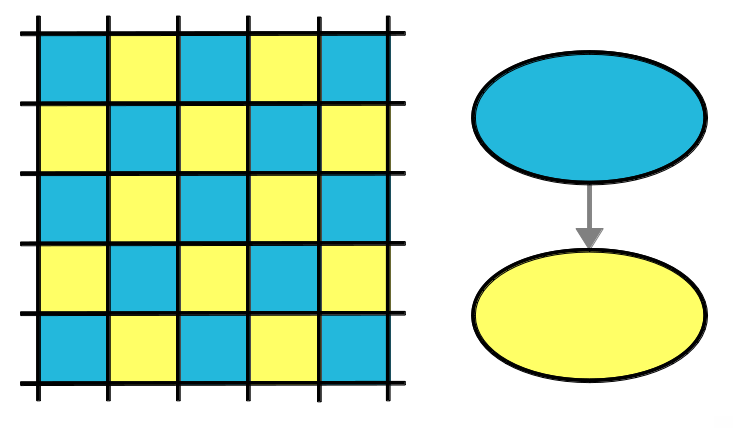
\includegraphics[scale=0.25]{Coloring_approach.png}
 \caption{Coloring approach}
\end{figure}

 \item COO (GlobalNZ)
 \item Hybrid COO/CSR with partitioning (sharedNZ)
 \item LocalNZ : redundant computations
 \item Atomics
 \item Unstructured Mesh Code Parallel Implementation
 \item Task Based Parallelisation SpMV, dongara and co \cite{MPI_task}
\end{itemize}

\section{Dassault Application : DEFMESH}

CFD, what for, how, current implem, mpi scalability ok...

3 versions L, NL, elas, nice picture of mesh deformation comparing the three variant

L, linear one step of deformation

NL, non-linear, the defamation is split into N small deformation, the mesh is updated after each deformation

elas. elasticity, like nl but with a more complex assembly step and different boundary condition for the solver ? the rational is to smooth the deformation (???)


explain the difference for the assembly step L,NL, vs alas

Test cases size and particularity (inc. numerical ?)



\section{Divide and Conquer}

The main idea of the Divide \& Conquer approach for shared memory parallelization is to create task level parallelism while preserving a good data locality and
minimizing synchronization cost. It is based on a topological recursive bisection of the mesh.

Since the newly created sub-domains are not sharing any element, they can be treated in parallel.
However, elements on the frontier have nodes in both sub-domains and must be treated after they completed.
Therefore it is important to use a good partitioner to build equal sub-domains while minimizing the interface. In our case, we use the METIS graph partitioner.
This partitionment is illustrated in the figure below.
\begin{figure}[htp]
 \centering
 \label{fig2}
 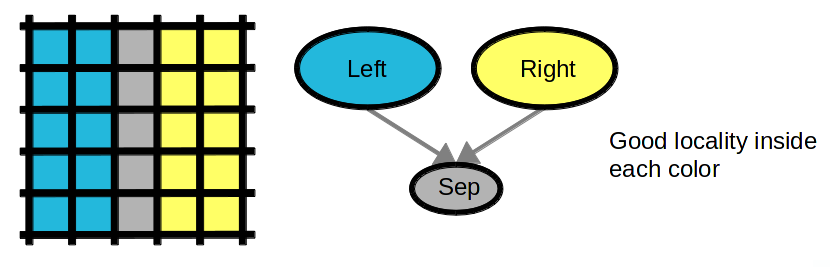
\includegraphics[scale=0.25]{DC_approach.png}
 \caption{Coloring approach}
\end{figure}
All the sub-domains are split recursively, offering a large amount of parallelism.
This process results in a recursive partition tree where each leaf is associated with an independent Cilk task.
For each node of this tree, the intervals of nodes, elements and separators used at the current step of recursion are stored.
This tree is represented in the figure below.

The Cilk implementation is then straightforward. Execution runs through the tree starting from the root and spawning a new Cilk task at each node separation.
This creates at each step of recursion parallelism between left and right parts.
Then, when recursion reaches a leaf, the code is simply running the sequential assembling on its sub-domain.
After left and right sub-domains are done, the corresponding Cilk tasks synchronize and one of them continue on the separator computation.
\begin{figure}[htp]
 \centering
 \label{fig3}
 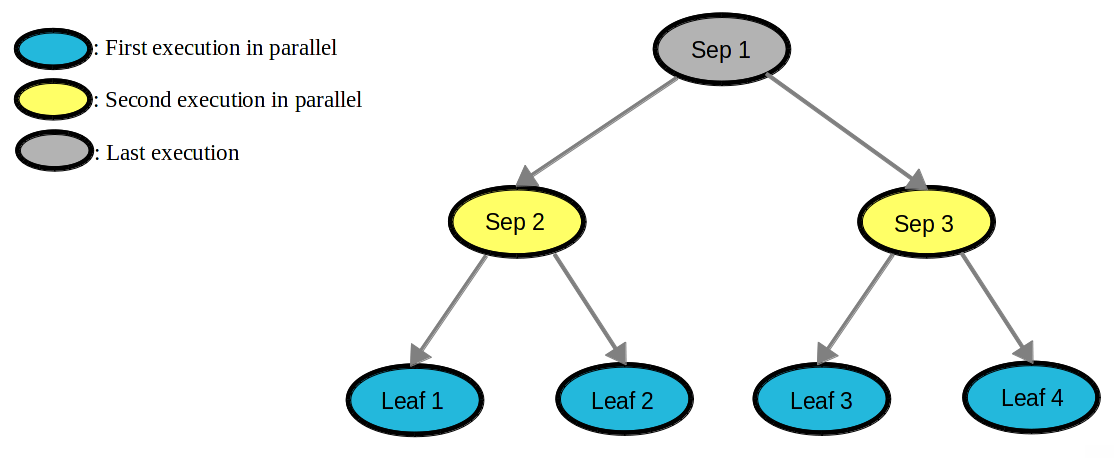
\includegraphics[scale=0.25]{Recursion_tree.png}
 \caption{Coloring approach}
\end{figure}
In order to increase the data locality, we permute the nodes and the elements arrays. Indeed the elements can be consecutive in memory inside each sub-domain,
improving intra-task locality.
Secondly, since the tasks distribution is following the recursive domain decomposition, we store neighbor sub-domains and associated separator contiguously to improve
locality between tasks. Some other data structures have to also be permuted or renumbered in order to be compatible with the MPI decomposition and the other inputs.
Some of them are for instance the solution arrays or the interfaces between MPI domains.
This storage is illustrated in the figure below.
\begin{figure}[htp]
 \centering
 \label{fig4}
 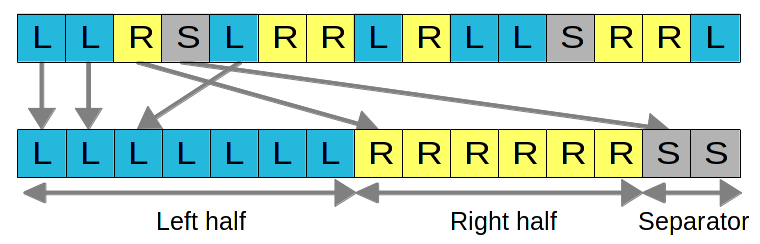
\includegraphics[scale=0.25]{Data_permutations.png}
 \caption{Coloring approach}
\end{figure}
Otherwise, since the partitionment is topological, cuts are done on edges and not on geometrical coordinates. This allows to compute the sub-domains only once
for a given mesh, despite of its deformations. Thus, the METIS partitioning and the creation of permutations arrays and recursion tree can be done only once.
These structures have simply to be stored for instance with the mesh. On following runs, the application needs only to read these data and apply the permutations.

\begin{itemize}
 \item introduction of the following subsection
 \item locality (data, sync) and concurrency for efficient parallelisation
 \item nice figure to explain separation LRS and nice mesh figure (from specfem?)
 \item explain the pb of knowing where to write the data (better data structure?)
 \item explain the pb of identifying the concurrency, sort so that subdomain are independent, explain why it helps data locality
 \item separator
 \item Matrix assembly
 \item Solver, conjugate gradient, ddot, spmv, reduction
 \item Communication for halo exchange
\end{itemize}


\subsection{Unstructured Domain decomposition}

metis explain how why space filling curve etc.

Explain the result, the reordering of the data, and the renumerotation of the interface to have a minimal intrusion on the original code.
(talk about elision, silk elision, our code in Fortran elision)

The Initial mesh coordinate array is firstly tranform in a nodal graph thanks to METIS before decomposing it. Indeed, METIS recursive partitioning routine works directly
on a graph, dual or nodal. We use nodal one because we need to partition both nodes and elements but also make a distinction between elements wich are fully composed of
nodes in a same partition and those which are on the separation of two node partitions. This option is not provided with dual graph decomposition METIS.
METIS also proposes a "meta-function" of mesh partitioning wich combines mesh to graph transormation and graph partitioning, but we experiment better performances by
calling separatly this two functions.
The final output is an array, dimensionned to the number of nodes in our mesh, which indicates the partition number of each node.
Starting from this node partition array, we can compute an element partition array associating each element to the same partition number than their nodes.
If an element is composed of nodes from two or more partitions, it is called a separator and it belongs to a distinct partition number.
Thanks to this partition arrays on resp. elements and nodes we can easily compute two permutation arrays on resp. elements and nodes giving for each of them, their new
index in the initial mesh arrays. We apply these permutations on the coordinate array (x,y,z of each node), on the "element to node" array and on the reference solution.
We also have to renumber each node of the "element to node" array in order to stay coherent with the newly permuted coordinate array. For the same reason we permute the
interface array, listing the nodes at the separation of two sub-domains and exchanged by MPI process. (and ?)

\subsection{Cilk implementation of task tree}

Cilk is a task based runtime working on threads. It allows to create parallel tasks with the \emph{spawn} keyword and to synchronize them with the \emph{sync} keyword.
Tasks are executed by Cilk \emph{workers}. Each core is linked to a worker which executes a new tasks as soon as it can.
Cilk runtime uses a work-stealing scheduler to dynamically load-balance the tasks. Each worker has a queue of tasks to execute.
Once a worker completes all its tasks, it can steal others from slower workers.

explain why we want task base runtime, load balancing, fine grain...

explain problematic of sync, conherency, vecto etc.


Implementation of the tree to call and sync.

indirect access to vertices local to an element

stop when ???

Once the data permuted and renumbered, we create a recursion tree giving for each step of partitionment the interval of nodes used, of elements belonging to left subdomain,
right subdomain and the interval of separator elements belonging the subdomain at the frontier of left and right ones.
Thus, the tree root intervals contain all  the nodes of the mesh, and all the elements separated in 3 parts (LRS) and the leaves of the tree contain just the necessary nodes
for their subdomain and the interval of elements used (no more separator or left and right distinction).
Once the recursion tree is done, we just have to recursivly run through it from the root to the leaves and spawning a new cilk task at each node until we arrive at the maximum
number of tasks fixed or at the end of the tree. If we stop at a leaf, the corresponding cilk task will simply do the mesh assembling on its independant subdomain of nodes and
elements. If we stop earlier at a node, the corresponding tasks will perform the assembly on its left and right half (stored contiguously in memory) and the on its separator
part (stored also contiguously). Once this leaves or nodes are computed, we go back in the tree and compute the separator subdomains of each parent nodes.
Sepator subdomains are not yet decomposed (futur work) and can represent for the moment an incompressive part non negligible of the assembling step, especially the first
separator subdomain at the root of the tree.

\subsection{Parallel for}

when all element access in order, no need of task tree: cilk for or openMP

If the solver step is prototyped talk about it with the list of basic operation given by Quang.

how it works, the parameters


\subsection{Cilk+MPI}

com has to be done once in sequential section, avoid com from mpi domain decomposition replaced by data sharing, take benefit of the machine topology


Result expected is on small number of core cilk+MPI == pure MPI, on larger number of core D\&C silk is expected to continue scaling

\section{Results}


Experiments have been done on the Dassault Aviation EIB test case. It is an irregular mesh composed of 6 346 108 elements and 1 079 758 nodes.
It represents the displacement of fuel tank along a plane fuselage.

In the following experiments, we compare two versions of the DEFMESH application: the original one from Dassault Aviation called “Ref” and the new
Divide \& Conquer version called “D\&C”. The original version uses MPI between the different blocks of the mesh and OpenMP in some loops of the solver.
The D\&C version, as described above uses a recursive partitioning of each block of the mesh and exploits, in addition to MPI and OpenMP, a Cilk task parallelism
in the assembly step.

For each of these versions, we consider the two different solvers of DEFMESH: the Laplacian one and the elasticity one.
Both of them are non linear solvers with 50 steps of resolution. Measures correspond to the average time of one iteration.
In all cases we measure separately the assembly step, where the D\&C approach has been applied and the solving step, not yet modified.

We present the results both in terms of execution times and of parallel efficiency.
In all the graphics, the X axis represents the number of cores used. It corresponds to the product of MPI ranks by the number of Cilk / OpenMP threads.
In execution times graphics, the Y axis correspond either to RDTSC cycles (assembly step) or MPI\_Wtime seconds (solving step).
Concerning efficiency, the Y axis represents parallel efficiency given by the following formula:

\emph{Efficiency on p cores = Time of the sequential algorithm / ( p * Time on p cores)}\\

Graphics include the measures of the “Ref” and the “D\&C” versions.
For each of them, we use 1, 4, 8 and 12 MPI tasks and from 1 to 12 Cilk and OpenMP threads while the combination of MPI processes per Cilk/OMP threads is lower or equal to 12,
which correspond to the number of cores available. In all cases, the number of Cilk threads is equal to the number of OpenMP threads.
We also varied the number of METIS partitions and Cilk tasks in a large scope of values but we have not observed significant changes in the results.
Final values are 512 partitions and 128 Cilk tasks. This correspond to approximately 10 tasks per core, which is recommended in Cilk documentations.

All the experiments have been done with default the OpenMP affinity set to scatter and Cilk threads are not pinned. These experiments runs on an UVSQ server
composed of twelve cores distributed in two sockets of 6-cores Intel® Xeon® X5650 clocked at 2.67 GHz. The topology of the machine is described in the following illustration.
\begin{figure}[htp]
 \centering
 \label{fig5}
 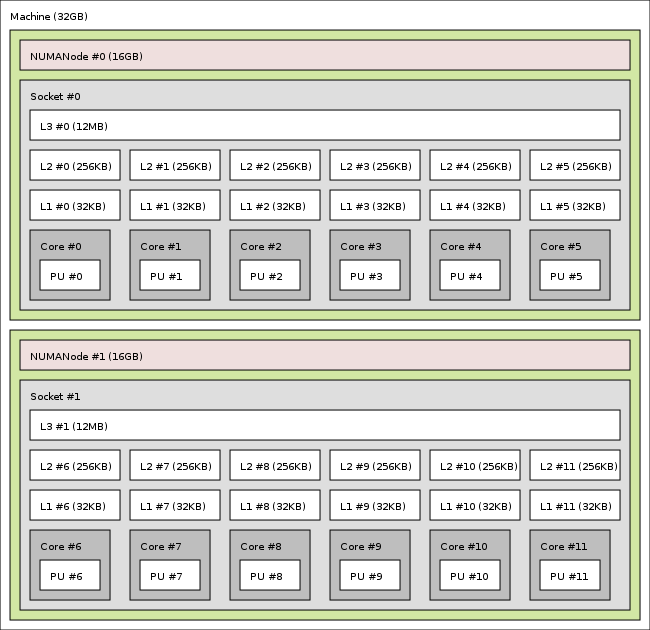
\includegraphics[scale=0.35]{topo_mauduit.png}
 \caption{UVSQ server topology}
\end{figure}

\subsection{Laplacian solver}
\emph{Assembly step}\\
\begin{figure}[htp]
 \centering
 \subfigure[Execution time]{\label{fig6:a}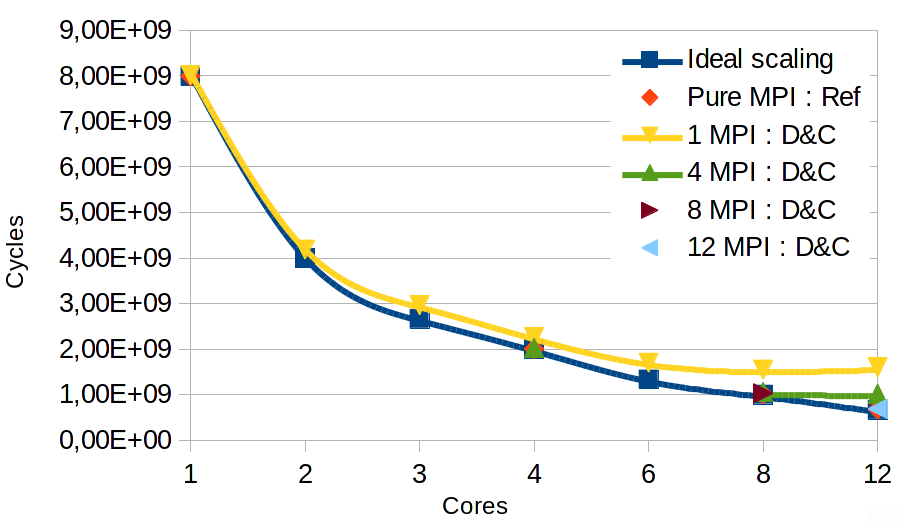
\includegraphics[scale=0.178]{Laplacian_asm_time.png}}\hspace{1em}%
 \subfigure[Parallel efficiency]{\label{fig6:b}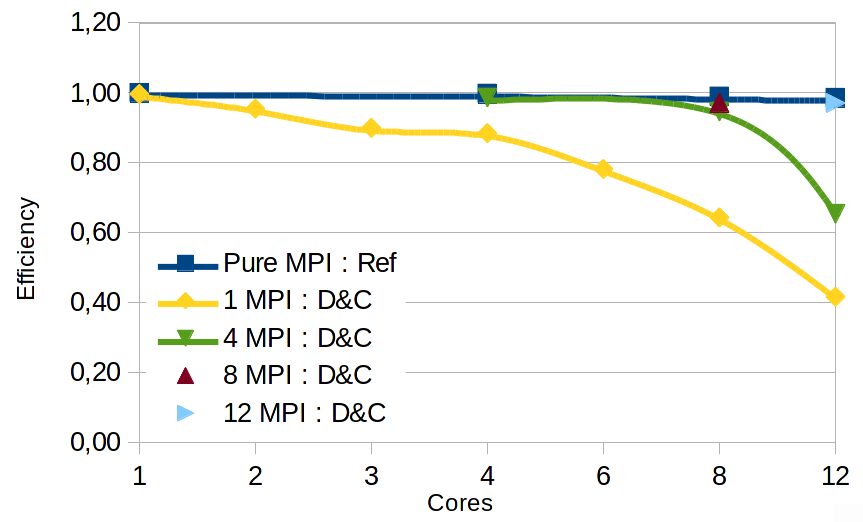
\includegraphics[scale=0.178]{Laplacian_asm_efficiency.png}}
 \caption{Laplacian assembly step}
\end{figure}

On the execution time curve, the D\&C approach is close to pure MPI but there is still a loss of efficiency beyond 6 cores.
This is probably due to the remaining sequential part of the D\&C code. Indeed, separator elements are not yet parallelized and can represent an important proportion
of the computation, especially for the one at the beginning of the recursion.

As we can see on the efficiency curve, the more the number of cores increase, the more the efficiency decrease. According to the Amdahl law,
the proportion of the sequential part over the parallel part is increasing with the number of cores. Moreover on the Laplacian solver, the amount of work for each
element in the assembly step is quite low and separators even less negligible. In the pure MPI version, this problem is not present since the whole mesh assembly is parallelized.

All in all, these first results are encouraging and we can reasonably expect to match the ideal scaling when the separators will be parallelized.

\emph{Solving step}
\begin{figure}[htp]
 \centering
 \label{fig7}
 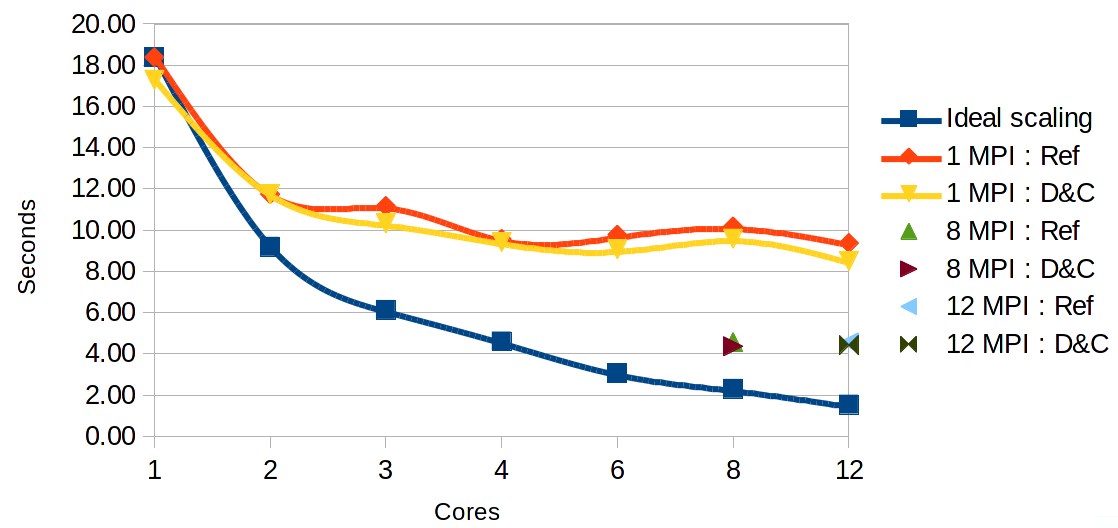
\includegraphics[scale=0.2]{Laplacian_solver_time.png}
 \caption{Solver execution time}
\end{figure}
The gains offered by the OpenMP parallelism are far from ideal scaling because of the small proportion of code parallelized in the solver.
Despite we did not modify the solver part, we observe a small benefit for the D\&C version compared to the reference version.
This gain is probably due to a better data locality generated by the permutations as explained in the previous section.
To confirm the locality hypothesis, we measured the L3 cache misses occurring during the solver and they are significantly lower with D\&C compared to the original version.
We also tried to permute data randomly and observe a degradation of performances.

\subsection{Elasticity solver}
\emph{Assembly step}\\
\begin{figure}[htp]
 \centering
 \subfigure[Execution time]{\label{fig8:a}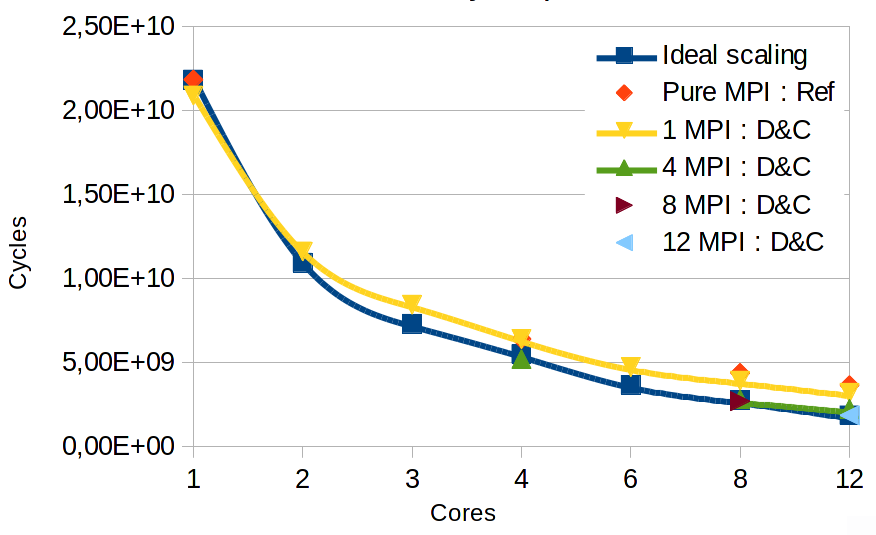
\includegraphics[scale=0.19]{Elasticity_asm_time.png}}\hspace{1em}%
 \subfigure[Parallel efficiency]{\label{fig8:b}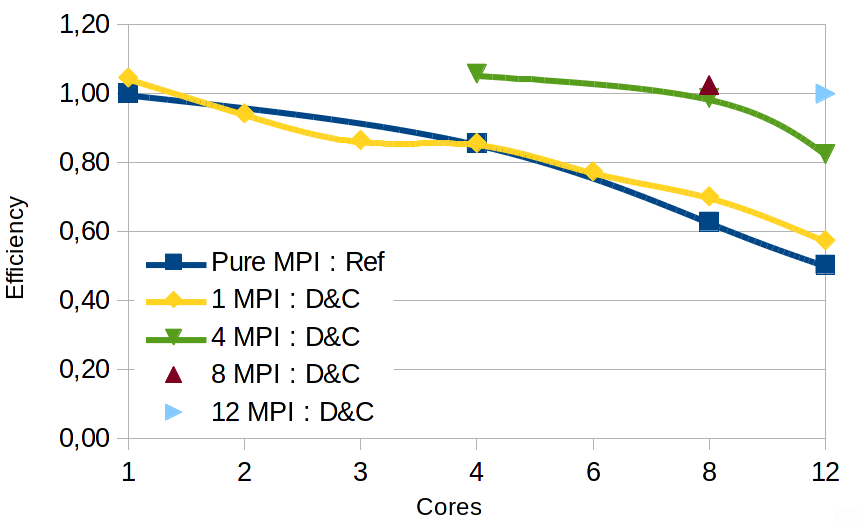
\includegraphics[scale=0.19]{Elasticity_asm_efficiency.png}}
 \caption{Elasticity assembly step}
\end{figure}

As we can see on the first curve, on the elasticity solver the D\&C approach is slightly faster than pure MPI and the parallel efficiency is equivalent.
In the elasticity case, the amount of work of the assembly step is bigger than the Laplacian.
Thus, the sequential part (ie separators computing) is less significant and the D\&C scalability gets better beyond 6 cores.
Moreover in the D\&C version, data continue to fit in cache whereas MPI starts to slow down. Indeed, where the original version works on elements located
anywhere in the current MPI block, the D\&C version works on elements packed contiguously in small blocks corresponding to the Cilk tasks.
With this approach, whatever the size of the data set, the tasks will always fit in cache if we increase the number of METIS partitions.\\

\emph{Solving step}
\begin{figure}[htp]
 \centering
 \label{fig9}
 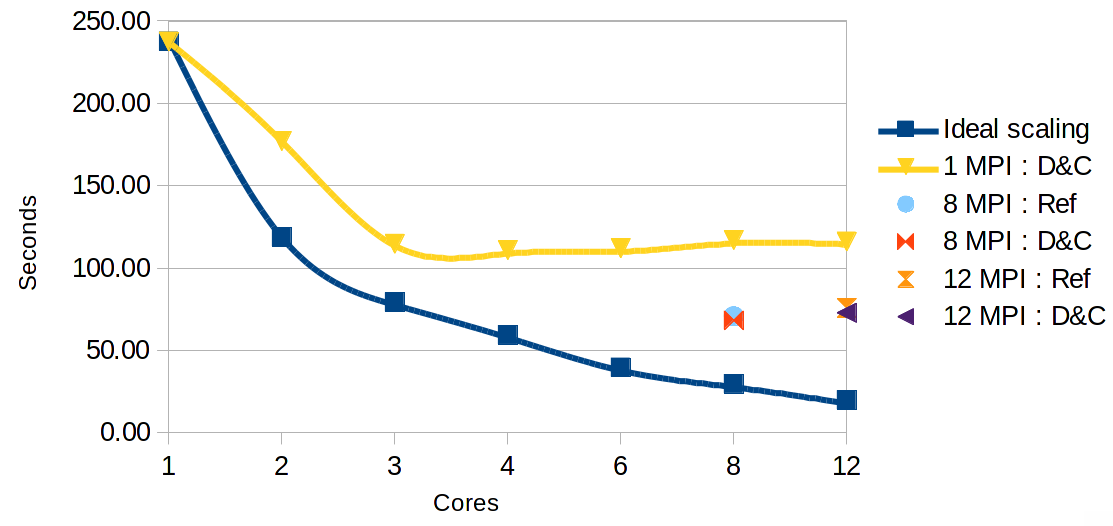
\includegraphics[scale=0.2]{Elasticity_solver_time.png}
 \caption{Solver execution time}
\end{figure}
As we can see in the 4 MPI curves and for the same reasons than in the Laplacian solver, the D\&C version is still a little bit faster than the original version.
We can expect even better results when the solver will be properly parallelized.
Further investigation are needed to evaluate why the pure MPI version does not scale perfectly in our experiments.

\subsection{Sequential}
\subsection{Coloring}
\subsection{D\&C}

scalability cilk small test case

scalability cilk +MPI small test case, big test case


replace on a 32 core machine 32MPI by 4MPI*8cilk or 2MPI*16cilk or 1 MPI *32 silk etc.

replace on a 2node *16 core   ...... excpt 1 MPI...

replace on 4 node*8core ........ except 2 and 1 MPI...


locality: miss rate (does not work yet) , estimating data reuse with counters

\section{Conclusion and Futur Work}

Assembling is only the 5 first percent of the app, but this is the starting point. reprints large time in other some other mesh deformation code such has seismic
simulation like specfem3D.
HW counter already show that vertex and element reordering bring septential improvement on data locality. We also show a global improvement on RAM usage (?) etc...
The next step will be to work on the solver stage, using similar printiple to enhance scalability and efficiency. Explore D and C friendly data structure because CSR sucks.  

Extension will focus on D\&C friendly data structure definition, using D\&C on other part of the  application such as the spMV product or the iterative solver. 

Can we do something quick about spmv? we have some material on it...

\bibliographystyle{unsrt}
\bibliography{dc_bib}

\end{document}
